\chapter{Implementazione}\label{ch:implementazione}
\section{Scala 3}\label{sec:scala-3}
In questa sezione vengono esaminati in che modo e dove sono stati utilizzati i nuovi costrutti di Scala 3 nel progetto.

\subsection{Impliciti}\label{subsec:impliciti}

\subsection{Macro}\label{subsec:macro}

\subsection{Context function}\label{subsec:context-function}

\subsection{Match types}\label{subsec:match-types}

\subsection{Type class}\label{subsec:type-class}

\subsection{Extension method}\label{subsec:extension-method}

\subsection{Problemi riscontrati}\label{subsec:problemi-riscontrati}
Nella libreria \texttt{scalatest} è stato riscontrato un bug nel costrutto \texttt{shouldNot typeCheck}.
Questo consente di verificare che un'espressione, definita come stringa, non passi il controllo del type
checker e di conseguenza non compili.
Questo controllo risulta utile nel verificare il corretto "unpacking" delle \texttt{CList}: nello specifico si è testato
che un unpacking che contiene più elementi di quelli contenuti nella \texttt{CList} non compili;
a tal proposito si è definito il test indicato nel Listato~\ref{lst:lstinputlisting22}:
\lstinputlisting[label={lst:lstinputlisting22}, caption=Test per la verifica dell'unpacking delle CList.]
{./code/scalatest-bug.scala}
Nella prima asserzione si verifica l'unpacking con meno elementi di quelli nella \texttt{CList};
nella seconda si testa lo scenario opposto, quindi l'unpacking con più elementi di quelli presenti nella \texttt{CList}.
Per entrambi i due scenari appena descritti, la compilazione deve fallire a causa di un mismatch di tipi.
Tuttavia questo non accade poiché in entrambi i casi le espressioni vengono valutate erroneamente come valide.
Il bug è stato segnalato agli sviluppatori della libreria mediante una issue~\cite{scalatest-bug}.

Sin dalle prime fasi di sviluppo si è abilitata la modalità di \textit{cross-building}~\cite{cross-building} affinché il
framework venisse compilato anche per Scala.js~\cite{scalajs}.
Questo ha generato una serie di falsi errori all'interno dell'IDE (IntelliJ);
infatti se si eseguivano i comandi di Sbt per la compilazione del progetto, quest'ultimo non sollevava alcun errore.
tanto è vero che se si eseguivano i comandi di Sbt per la compilazione del progetto, quest'ultimo non sollevava alcun
tipo di errore.
A tal proposito è stata aperta una issue~\cite{intellij-issue} sul bug tracker di Jetbrains.
Per una maggiore agilità nella scrittura del codice si è quindi scelto di rimuovere la \textit{cross-building} dal
progetto.

Si segnala che, essendo il rilascio di Scala 3 relativamente recente, non è stato possibile utilizzare
le seguenti librerie per problemi di compatibilità:
\begin{itemize}
    \item Scalafix
    \item Scoverage
    \item ScalaFXML
    \item ScalaMock
\end{itemize}

\section{Benchmarks}\label{sec:benchmarks}
Il requisito non funzionale~\ref{itm:nf1} richiede che il framework operi sotto certi requsiti di prestazioni;
per questo motivo occorre quantificare con dati oggettivi quali siano le effettive prestazioni raggiunte.
I benchmark sono uno strumento piuttosto efficace e preciso per valutare i tempi di esecuzione (e non solo), fornendo
una stima accurata delle prestazioni in gioco.

Con il termine benchmark si intende un insieme di test specifici per misurare le prestazioni di un software o computer.
Al termine dell'esecuzione del benchmark si ottiene un indice indicativo delle prestazioni che il sistema in oggetto ha
raggiunto.
I benchmark possono essere raggruppati in due categorie:
\begin{itemize}
    \item Sintetici (o microbenckmark): vanno a misurare le prestazioni di alcune parti specifiche di un sistema
    \item Applicativi: misurano le prestazioni complessive di un sistema, ad esempio di un'applicazione
\end{itemize}

Dal momento che si vogliono valutare solo le prestazioni di una specifica parte del framework si è deciso di effettuare
dei microbenchmark.

Per implementare tali benchmark si è fatto uso del framework \texttt{Jmh}~\cite{jmh}, il quale consente di definire in
modo piuttosto semplice ma altamente configurabile i benchmark.

Scrivere benchmark che misurano correttamente the prestazioni di una piccola parte di software è difficile.
Ci sono diverse ottimizzazioni che la JVM e l'hardware sottostante sono in grado di fare quando il benchmark esegue il
componente.
Tali ottimizzazioni non possono essere effettuate quando il componente è eseguito come parte dell'intera applicazione.
Implementazioni errate di benchmark possono far credere che le prestazioni dei componenti siano migliori di quanto non
saranno in realtà.

Scrivere un benchmark corretto tipicamente evita che la JVM e l'hardware sottostante effettuino ottimizzazioni
durante l'esecuzione del benchmark, ottimizzazioni che potrebbero non essere effettuate a livello complessivo di
applicazione.
Grazie a Jmh tutte queste configurazioni sono fatte in automatico e gestite direttamente dal framework, consentendo di
concentrarsi solamente su cosa deve essere testato.

Mediante l'utilizzo di annotazioni sulle classi e metodi è possibile configurare uno o più benchmark: nel
Listato~\ref{lst:lstinputlisting4} è possibile osservare un esempio di configurazione di un benchmark.

\lstinputlisting[label={lst:lstinputlisting4}, caption=Codice per eseguire il setup di un benchmark.]
{code/benchmark.scala}

Come è possibile osservare dal listato, Jmh fornisce molteplici configurazioni che possono essere apportate al
benchmark.
Di particolare rilevanza troviamo: \texttt{@Warmup} e \texttt{@Measurement}.

Con la prima si specifica quante iterazioni devono essere eseguite "a vuoto" prima d'iniziare con i test effettivi;
questa procedura risulta necessaria dal momento che quando si esegue per la prima volta un programma sulla JVM, la cache
risulta vuota e quindi il caricamento iniziale delle classi risulta più lento.
Eseguendo più volte la stessa porzione di codice si "stabilizza" la cache, quindi gli accessi successivi saranno più
veloci e uniformi nei tempi.
In questo modo si garantisce che le misurazioni successive alla fase di warm up abbiano valori simili senza essere
influenzate da condizioni esterne.

Con la seconda si specifica quante esecuzioni devono essere effettuate del benchmark.
Per ogni esecuzione viene annotato il tempo impiegato e al termine dell'esecuzione viene riportato il tempo medio che
impiega il test.

\subsection{Risultati}\label{subsec:risultati}
Di seguito sono analizzati i risultati ottenuti dai benchmark delle \View e dei \System.
In Figura~\ref{fig:system} viene mostrato il grafico riguardante i \System in cui si può osservare che con $10000$
entità un sistema impiega mediamente cinque millisecondi ad aggiornare le entità, quindi il requisito~\ref{itm:nf1} è
ampiamente rispettato.

\begin{figure}[H]
    \centering
    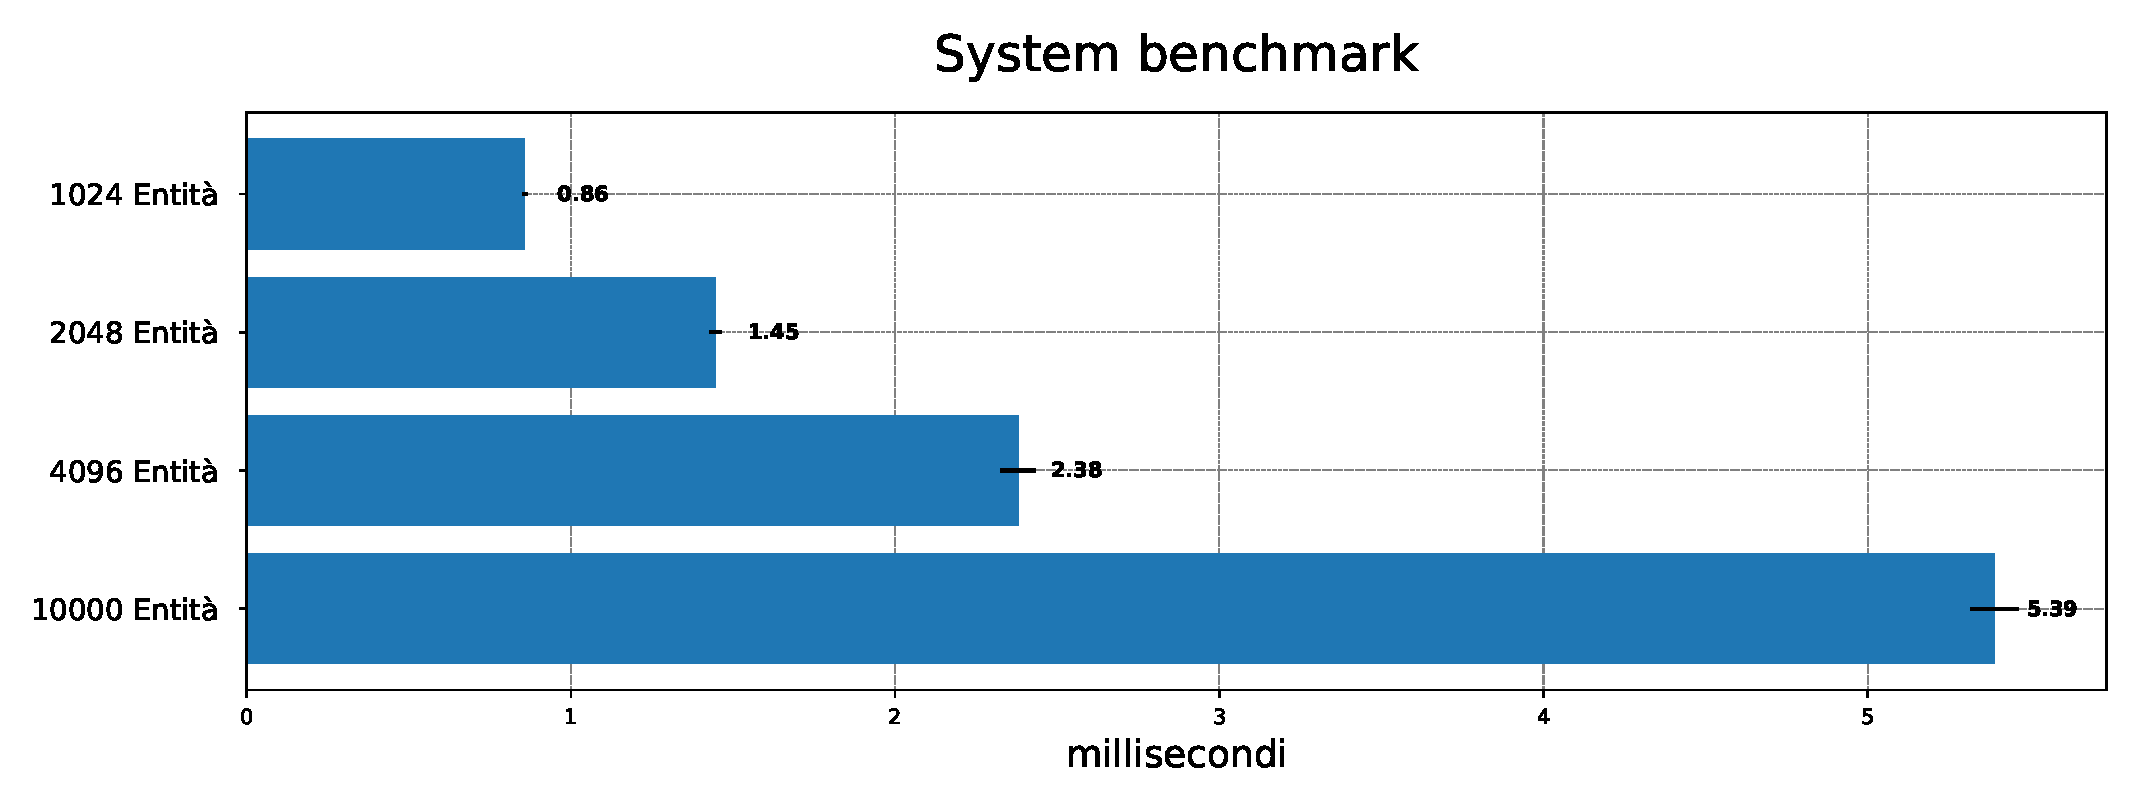
\includegraphics[width=\textwidth]{./img/system-benchmark}
    \caption{Tempi di esecuzione di un \System}\label{fig:system}
\end{figure}

A fronte dei risultati ottenuti dai benchmark si può affermare che il framework fornisce buone prestazioni con un numero
piuttosto elevato di entità.

\section{Suddivisione del lavoro}\label{sec:suddivisione-del-lavoro}
In questa sezione viene illustrata la suddivisione del lavoro e le parti di progetto realizzate da ciascun membro del
gruppo.

\subsection{Farabegoli}\label{subsec:farabegoli}
Il contributo apportato al progetto ha toccato buona parte del core del framework e della demo.
Mi sono infine occupato della gestione del repository, della \textit{Continuous Integration}, dei rilasci del framework
e della qualità del codice.

\subsubsection{Sviluppo collaborativo}
Spesso mi sono trovato a lavorare assieme ad altri membri del gruppo per risolvere problematiche o fornire spunti per
un migliore sviluppo del codice.
A tal proposito sono state frequenti le sessioni di lavoro in \textit{pair programming} che ci hanno consentito di
superare velocemente difficoltà nell'implementazione del codice, oltre a intercettare fin da subito potenziali bug.

\subsubsection{Component list}
La necessità di creare una tipologia di liste che contenesse al suo interno elementi di tipi diversi è nata dal fatto
che si vuole sfruttare il generico per specificare su quali~\Component devono operare i \System (e le \View).
L'utlizzo delle liste convenzionali non è sufficiente in quanto essendo covarianti, quando si accede a un elemento della
lista, questo viene ritornato con il sopratipo comune della lista e non con il tipo effettivo inserito.
Si vuole quindi creare un costrutto che garantisca un livello maggiore di astrazione, mantenendo tutti gli aspetti
di type-safety noti delle liste, e che consenta anche di memorizzare elementi con tipi differenti nella stessa
collezione.
A tal proposito mi sono occupato della realizzazione delle \texttt{CList} per rendere i \System \textit{type-safe}
intercettando tutti gli errori dell'utente a compile-time.
La peculiarità di questa lista è data dal fatto che gli elementi in essa contenuti possono essere di tipi differenti:
questa costruzione prende il nome di~\textit{heterogeneous list}.
La costruzione delle \texttt{CList} è ispirata alla libreria \texttt{shapeless}~\cite{shapeless}.

Nel Listato~\ref{lst:lstinputlisting} viene riportata una versione semplificata d'implementazione delle \texttt{CList}.
\lstinputlisting[label={lst:lstinputlisting}, caption=Esempio di codice per implementare CList.]{code/clist.scala}

Nel contesto del framework si vuole aggiungere il vincolo tale per cui gli elementi presenti nelle \texttt{CList} siano
sottotipo di \Component.

Oltre all'implementazione, mi sono occupato anche dello sviluppo dei test delle \texttt{CList}: un testing approfondito
si è reputato fondamentale poiché questo costrutto rappresenta un elemento chiave dell'intero framework.
Vista la rilevante importanza del testing per questo costrutto, una parte dei test sono stati condotti assieme agli
altri membri del gruppo affinché si potessero identificare tutti i possibili casi di fallimento da intercettare.
Durante lo sviluppo dei test sopracitati si è rilevato un bug nella suite \texttt{scalatest}; si veda la
Sezione~\ref{subsec:problemi-riscontrati} per una trattazione dettagliata del problema.

Il vantaggio offerto dalle \texttt{CList} è dato dal fatto che si può definire una lista di tipi e quindi utilizzarla
come tipo nelle funzioni che accettano un generico;
a tal proposito è stato possibile implementare \System e \View affinché accettino una \texttt{CList} nel
generico e quindi effettuino le operazioni solo sui tipi in essa definiti.

In Figura~\ref{lst:lstinputlisting2} viene mostrato un esempio di utilizzo delle \texttt{CList} nelle~\texttt{View}.
\lstinputlisting[label={lst:lstinputlisting2}, caption=Esempio di utilizzo delle CList.]{code/clist-usage.scala}

L'ordine dei tipi che definiscono una \texttt{CList} è fondamentale ai fini della computazione dei \System poiché se non
venisse rispettato si avrebbero inconsistenze di tipi che porterebbero a una condizione di errore che si vuole evitare.
Ciò consente nelle implementazioni dei \System o delle \View d'identificare a tempo di compilazione se la
\texttt{CList} che viene ritornata ha lo stesso tipo di quella dichiarata nel sistema;
se ciò non accadesse, il compilatore segnala un errore d'inconsistenza di tipi.
In questo modo garantiamo che un errato utilizzo delle \texttt{CList} venga intercettato a compile time, oltre a
preservare la semantica di utilizzo.

\subsubsection{World ed Entity}
Una delle parti che ho seguito nelle prime fasi di sviluppo è stata l'implementazione del \World e delle \Entity.
In particolare mi sono occupato di definire l'interfaccia di entrambe le classi e di fornire una prima implementazione
di base.
Ho quindi implementato la logica delle \Entity affinché, in fase di generazione, avessero tutte un identificativo
univoco nel \World.
Mi sono quindi occupato dello sviluppo dei test per la verifica delle classi oggetto d'implementazione.

\subsubsection{View}
Mi sono occupato di definire e implementare parzialmente la classe~\View.
Nello specifico mi sono occupato di definire l'interfaccia e fornire una prima implementazione della stessa.
Infine ho definito i test case necessari ai fini del testing della classe.
Sempre nell'ambito dello sviluppo delle \View, Cavalieri ha sviluppato una macro per costruire la \View in modo che
operi sui componenti effettivi passati nel generico;
in questa fase ho contribuito fornendo consigli e suggerimenti per una migliore implementazione del codice.

\subsubsection{Benchmarks}
Come descritto nel requisito non funzionale~\ref{itm:nf1} si vuole ottenere un certo livello di prestazioni dal
framework.
A tal proposito ho definito una serie di benchmark che vanno a quantificare le prestazioni ottenute.
Nello specifico ho definito due benchmark: uno per le \View e uno per i \System.
Mediante questi benchmark è stato possibile validare il requisito non funzionale sulla base di dati oggettivi.
L'aspetto di type-safety che garantiscono le \texttt{CList} è dato dal fatto che tutti i suoi componenti siano sotto tipo
di~\Component, quindi se viene costruita una~\texttt{CList} che comprenda un tipo che non è sotto tipo di~\Component,
allora l'errore viene intercettato a compile-time.

\subsection{Di Domenico}\label{subsec:nicolò-di-domenico}

Il mio ruolo nel progetto è stato principalmente quello d'implementare le \texttt{View} e i \texttt{System}, nonché
applicare ove necessario eventuali ottimizzazioni per rispettare il requisito non funzionale \ref{itm:nf1}.

\subsubsection{View}

Essendo le \texttt{View} ed \texttt{ExcludingView} progettate come indicato in Figura~TODO, si è rivelato utile costruire un
iteratore astratto che permettesse di fattorizzare tutto il codice comune.
In particolare si noti come la \texttt{ExcludingView} itera su un sottoinsieme delle entità ritornare dalla stessa
\texttt{View}, che invece non esprime vincoli di esclusione di componenti.
Per questo motivo è stato creato il \texttt{BaseViewIterator}, che si occupa di recuperare dal
\texttt{ComponentsContainer} tutte le mappe che associano ciascuna entità all'istanza (se presente) del componente di
ciascun tipo.
Infine, partendo da tali mappe, si occupa di testare l'appartenenza alla view di ciascuna entità e, in caso affermativo,
estrarne tutti i componenti richiesti.

Una semplice ottimizzazione utilizzata per rendere più veloce l'iterazione di una \texttt{View} consiste nell'individuare
la mappa di componenti con meno elementi;
una volta trovata, si iterano tutte le entità contenute al suo interno e per ognuna si controlla che sia presente in tutte
le altre mappe.
In caso affermativo, si procede all'estrazione di tutti i suoi componenti richiesti.

\subsubsection{System}

Un \texttt{System} è un blocco di codice che può essere aggiunto al \texttt{World} e viene chiamato a ogni aggiornamento
di stato della simulazione.
Ogni \texttt{System} ha due metodi:
\begin{itemize}
    \item \texttt{shouldRun}: metodo booleano che indica se il \texttt{System} dev'essere eseguito
    \item \texttt{update}: metodo che contiene il codice arbitrario da eseguire
\end{itemize}

Su di esso sono stati costruiti \texttt{IteratingSystem} ed \texttt{ExcludingSystem}, due wrapper type-safe
rispettivamente per \texttt{View} ed \texttt{ExcludingView}.
Questi due sistemi definiscono i seguenti metodi:
\begin{itemize}
    \item \texttt{shouldRun}: metodo booleano che indica se l'\texttt{IteratingSystem} dev'essere eseguito
    \item \texttt{before}: metodo eseguito prima di iterare su tutte le entità con i componenti richiesti
    \item \texttt{update}: metodo eseguito per ciascuna entità contenente le operazioni da effettuare sui suoi
    componenti richiesti
    \item \texttt{after}: metodo eseguito dopo aver iterato su tutte le entità con i componenti richiesti
\end{itemize}

Il metodo \texttt{update} deve ritornare una \texttt{CList} dei nuovi componenti;
grazie all'utilizzo delle \texttt{CList} (descritte in dettaglio in TODO) verrà verificato a tempo di compilazione che i
nuovi componenti abbiano lo stesso tipo di quelli su cui opera il sistema.
Per permettere la cancellazione di alcuni dei componenti, è stato implementato un \textit{match type} chiamato
\texttt{Deletable[L~<:~CList]}, come mostrato nel Listato~\ref{lst:deletable};
il suo scopo è quello di permettere l'inserimento in ogni posizione della \texttt{CList} un componente speciale chiamato
\texttt{Deleted}: in tal caso il componente in quella posizione sarà cancellato.

\lstinputlisting[label={lst:deletable}, caption=Implementazione del tipo \texttt{Deletable[L~<:~CList]}]{./code/deletable.scala}

L'\texttt{ExcludingSystem} è completamente analogo all'\texttt{IteratingSystem}, in quanto cambia solo la \texttt{View}
usata per ottenere le entità sulle quali iterare.
Per una maggiore più approfondita sui benchmark si faccia riferimento alla Sezione~\ref{sec:benchmarks}.